\documentclass[12pt]{article}

\usepackage[UTF8]{ctex}
\usepackage{appendix}
\usepackage{enumerate}
\usepackage{amsmath}
\usepackage{graphicx}
\usepackage{cite}
\usepackage{ragged2e}
\renewcommand{\raggedright}{\leftskip=0pt \rightskip=0pt plus 0cm}
\usepackage{array}
\usepackage{bigstrut}
\usepackage{geometry}
\usepackage{zhnumber}
\geometry{left =2.5 cm,right=2.5cm,top=2.5cm,bottom=2.5cm}
\usepackage{multirow}
\usepackage{lastpage}
\usepackage{longtable}
\usepackage{listings}
 \usepackage{color}
  \usepackage{xcolor}
  \lstset{
  language=Matlab,  %代码语言使用的是matlab
  rulesepcolor=\color{red!20!green!20!blue!20},%代码块边框为淡青色
  keywordstyle=\color{blue!90}\bfseries, %代码关键字的颜色为蓝色,粗体
    numbers=left, % 显示行号
    numberstyle=\tiny,    % 行号字体
   commentstyle=\color[RGB]{0,130,0},    % 设置代码注释的颜色
  showstringspaces=false,%不显示代码字符串中间的空格标记
  stringstyle=\ttfamily, % 代码字符串的特殊格式
  breaklines=true, %对过长的代码自动换行
  extendedchars=false,  %解决代码跨页时,章节标题,页眉等汉字不显示的问题
  escapeinside=``,      % 代码中出现中文必须加上,否则报错
  texcl=true,}
\usepackage[section]{placeins}
\usepackage[colorlinks,linkcolor=blue]{hyperref}
\usepackage{titlesec}
\usepackage{titletoc}
\titleformat{\section}{\heiti\zihao{3}}{\zhnum{section}、}{0.3em}{}
\titleformat{\subsection}{\heiti \fontsize{12pt}{0}}{\thesubsection}{0.3em}{}
\renewcommand\figurename{\heiti\zihao{5} 图}
\renewcommand\tablename{\heiti\zihao{5} 表}
\renewcommand {\thetable} {\thesection{}.\arabic{table}}
\renewcommand {\thefigure} {\thesection{}.\arabic{figure}}
\date{}
\geometry{a4paper,scale=0.8}

\begin{document}%文档从这里开始。

\numberwithin{footnote}{section}
\renewcommand{\contentsname}{\centerline{目录}}
\renewcommand{\tablename}{表}
\renewcommand{\figurename}{图}
\renewcommand\refname{参考文献}
\renewcommand\appendix{\setcounter{secnumdepth}{0}}
\renewcommand\abstractname{摘要}
\begin{figure}[h]
  \centering
  
\includegraphics[width=.6\textwidth]{logo}
\end{figure}
\thispagestyle{empty}
\begin{center}
\begin{songti}
\zihao{0}\textbf{音频放大器的制作}\\
\zihao{0}\textbf{设计报告}\\\ \\\
\zihao{3}
\\ \
\renewcommand\arraystretch{1.5}
\begin{tabular}{p{2.5cm}<{\centering} p{0.2cm}<{\centering} p{3.5cm}<{\centering} p{2.5cm}<{\centering} p{0.2cm}<{\centering} p{3.5cm}<{\centering}}
 课程&\textbf{:}&\multicolumn{4}{c}{电子系统综合设计与创新创业实践}\\\cline{3-6}
指导教师&\textbf{:}&\multicolumn{4}{c}{孙亚星}\\\cline{3-6}
组号&\textbf{:}&\multicolumn{4}{c}{第73组}\\\cline{3-6}
组员&\textbf{:}&常思克&学号&\textbf{:}&9161040G0313\\\cline{3-3}\cline{6-6}
组员&\textbf{:}&许晓明&学号&\textbf{:}&9161040G0734\\\cline{3-3}\cline{6-6}
组员&\textbf{:}&郭泽昊&学号&\textbf{:}&9161040G0919\\\cline{3-3}\cline{6-6}
组员&\textbf{:}&刘滔滔&学号&\textbf{:}&9161040G1021\\\cline{3-3}\cline{6-6}
组员&\textbf{:}&张锦涛 &学号&\textbf{:}&9161040G1034\\\cline{3-3}\cline{6-6}
\end{tabular}
\end{songti}
\end{center}
\begin{table}[b]
  \centering
\number\year\ 年\ \number\month月
\end{table}

\newpage
\zihao{4}
\newpage
\tableofcontents
\thispagestyle{empty}
\newpage
\setcounter{page}{1}

\setcounter{page}{1}
\section{设计说明}
\setcounter{equation}{0}
\setcounter{table}{0}
\setcounter{figure}{0}
\subsection{设计要求}
完成一个音频放大器设计制作,要求如下:
\begin{enumerate}
  \item 20dB增益
  \item 通带为1KHz~30KHz
\end{enumerate}
\subsection{系统组成}
根据设计要求,将音频放大器分为前置增益、低通滤波器和高通滤波器三部分,见图\ref{yuanli}
。\par
其中,由于要求20dB(10倍)的增益,设置前置增益的放大倍数为2倍、低通滤波器的通带放大倍数为2.5倍、高通滤波器的通带放大倍数为2倍。
\begin{figure}[htbp]
  \centering
  
\includegraphics[width=\textwidth]{picture/PPT1}
  \caption{音频放大原理框图}\label{yuanli}
\end{figure}
\section{子电路}
\setcounter{equation}{0}
\setcounter{table}{0}
\setcounter{figure}{0}
\subsection{前置增益:同相比例运算电路}
\subsubsection{电路原理}
如图\ref{txblyl}
\begin{figure}[htbp]
  \centering
  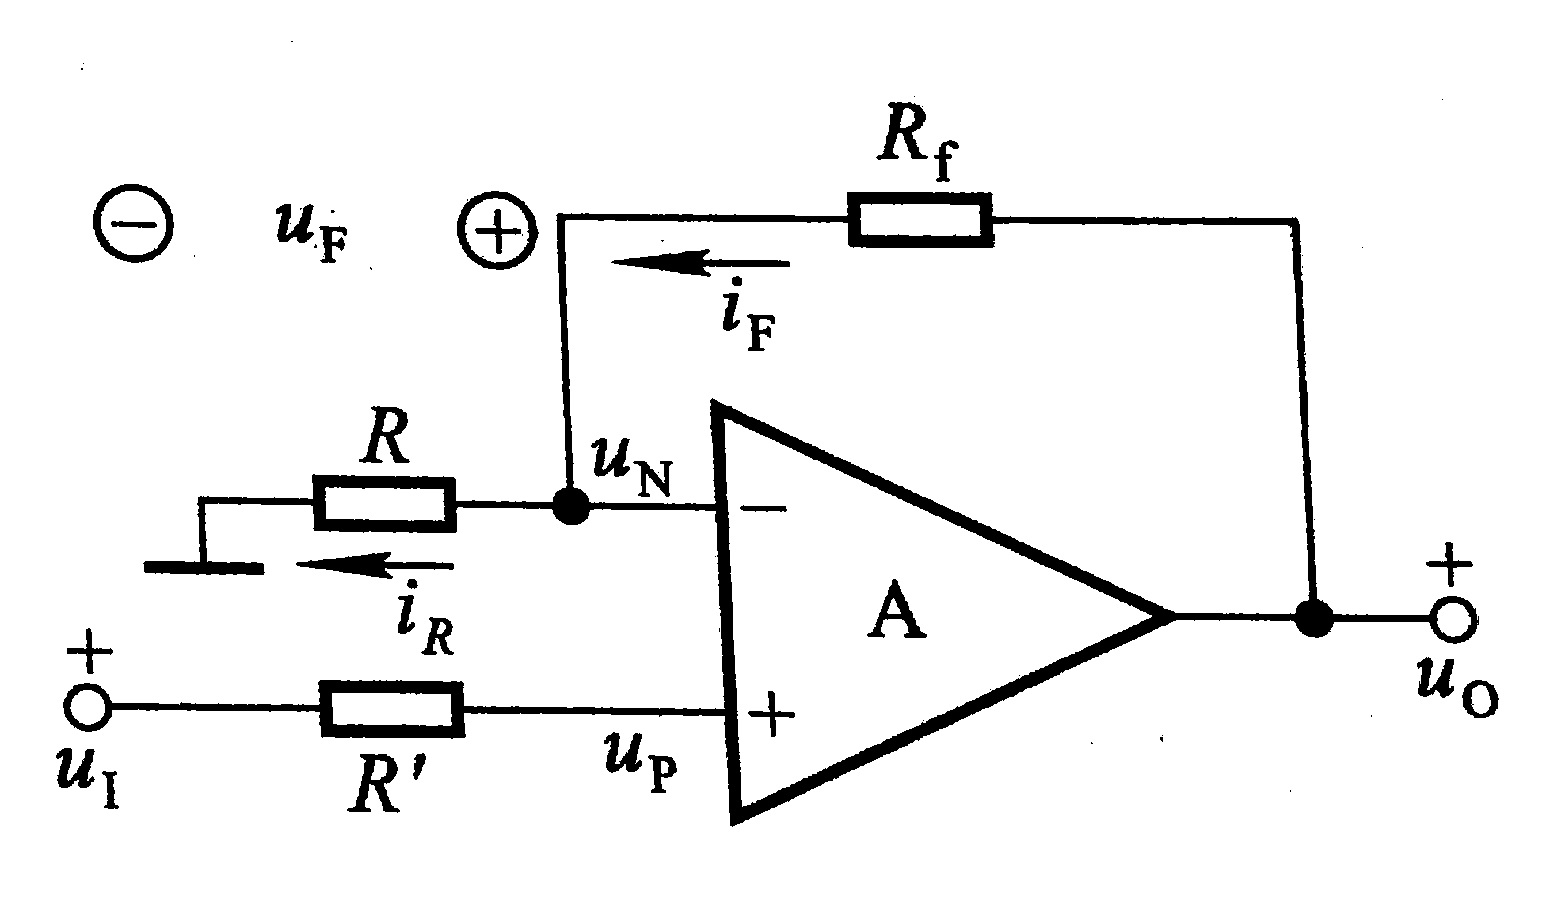
\includegraphics[width=.5\textwidth]{picture/P1}
  \caption{同相比例运算电路原理}\label{txblyl}
\end{figure}
,根据“虚短”和“虚断”,有
\begin{equation}\label{xuduan}
  u_P=u_N=u_I
\end{equation}
\begin{equation}\label{xuduan2}
  i_R=i_F
\end{equation}
即
\begin{equation}\label{tuidao1}
  \frac{u_N-0}{R}=\frac{u_O-u_N}{R}
\end{equation}
将式(\ref{xuduan})代入,得
\begin{equation}\label{jielun}
  u_O=\left(1+\frac{R_f}{R}\right)u_I
\end{equation}\par
为实现2倍放大,取$\frac{R_f}{R}=1$。
\subsubsection{Multisim电路图}
由电路原理,得到电路图如图\ref{qzzydlt}
。
\begin{figure}[htbp]
  \centering
  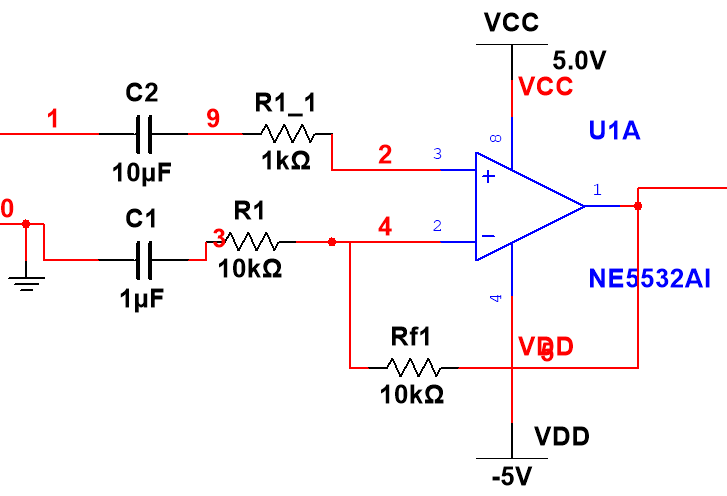
\includegraphics[width=.6\textwidth]{picture/TIM20190505123940}
  \caption{前置增益电路图}\label{qzzydlt}
\end{figure}
\subsubsection{仿真情况}
借助Multisim仿真,得到增益情况见图\ref{qzzyfzt1}
。\par 可知其基本符合2倍增益的要求。
\begin{figure}[htbp]
  \centering
  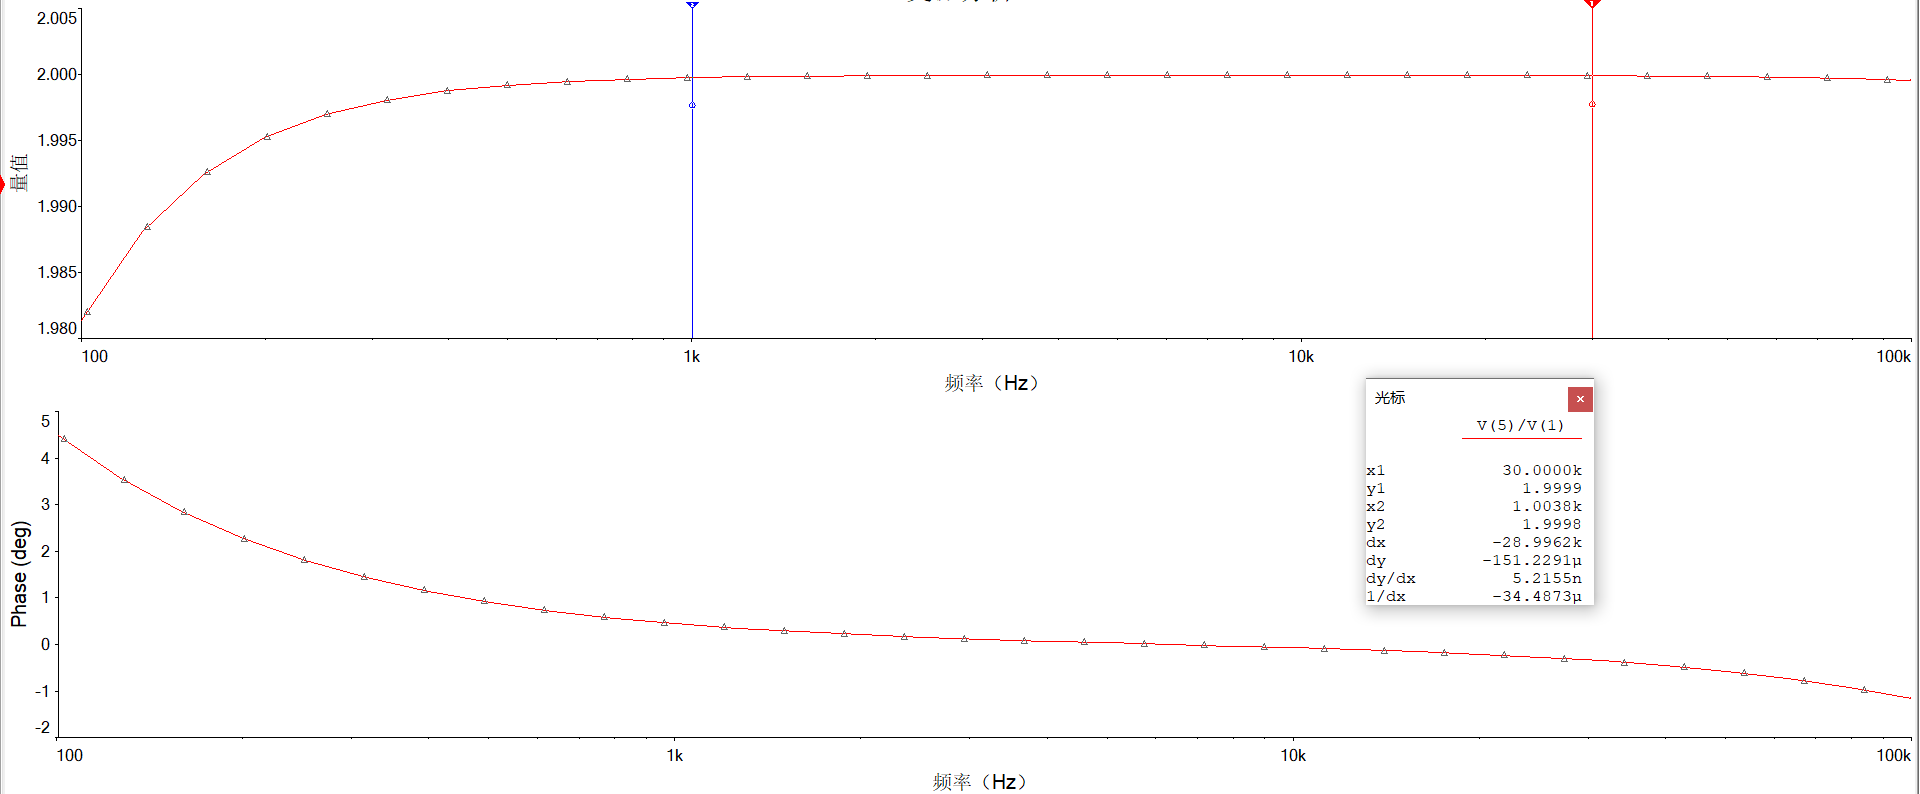
\includegraphics[width=\textwidth]{picture/TIM20190505124555}\\
  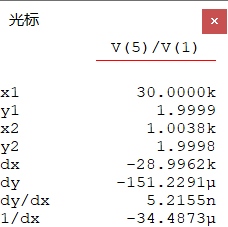
\includegraphics[width=.3\textwidth]{picture/TIM20190505124809}
  \caption{前置增益仿真情况}\label{qzzyfzt1}
\end{figure}
\subsection{同相输入一阶低通滤波器电路}
\subsubsection{电路原理}
如图\ref{yjdtlbq}
\begin{figure}[htbp]
  \centering
  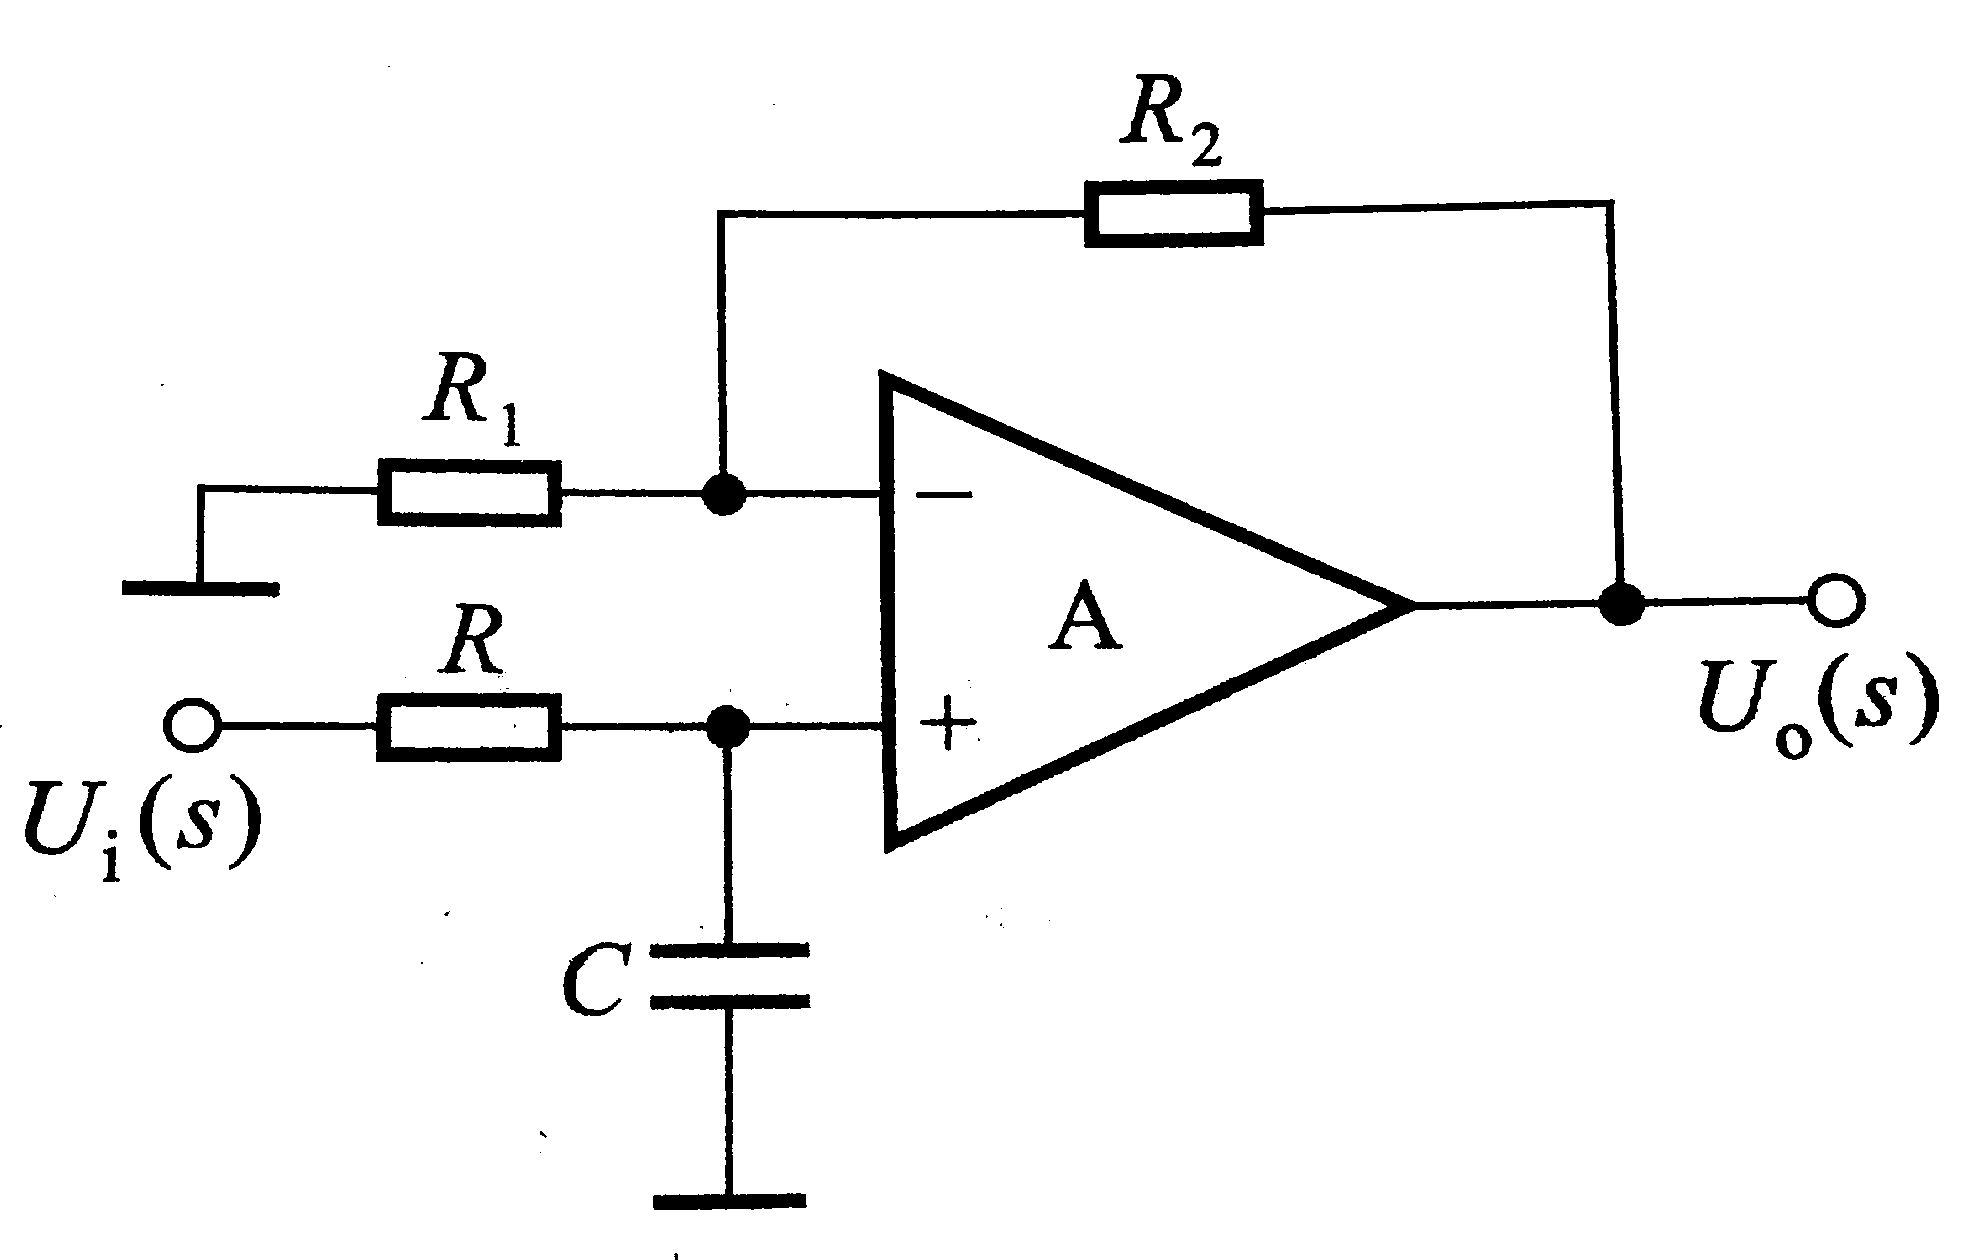
\includegraphics[width=.5\textwidth]{picture/P2}
  \caption{一阶低通滤波器电路原理}\label{yjdtlbq}
\end{figure}
,其传递函数为
\begin{equation}\label{cdhs}
  A_u(s)=\frac{U_o(s)}{U_i(s)}=\left(1+\frac{R_2}{R_1}\right) \frac{U_p(s)}{U_i(s)}=\left(1+\frac{R_2}{R_1}\right)\frac{1}{1+sRC}
\end{equation}
用$j\omega$取代$s$ ,且令
\begin{equation}\label{qudai}
  f_0=\frac{1}{2\pi RC}
\end{equation}
得到电压放大倍数
\begin{equation}\label{dyfdbs}
  \dot{A_u}=\left(1+\frac{R_2}{R_1}\right)\cdot\frac{1}{1+j\frac{f}{f_0}}
\end{equation}
其中,$f_0$称为特征频率。令$f=0$,可得到通带放大倍数
\begin{equation}\label{tdfdbs}
  \dot{A_{up}}=1+\frac{R_2}{R_1}
\end{equation}
当$f=f_0$时,$\dot{A_u}=\frac{\dot{A_{up}}}{\sqrt{2}}$ ,故通带截止频率
\begin{equation}\label{tdjzpl}
  f_p=f_0
\end{equation}\par
为实现2.5倍通带增益、3dB截止频率为30KHZ,取$\frac{R_2}{R_1}=1.5\mbox{,}f_p=30KHZ\mbox{,于是}R=2500\Omega\mbox{,}C=2.1nF$
\subsubsection{Multisim电路图}
由电路原理,得到电路图如图\ref{qzzydlt11}
。
\begin{figure}[htbp]
  \centering
  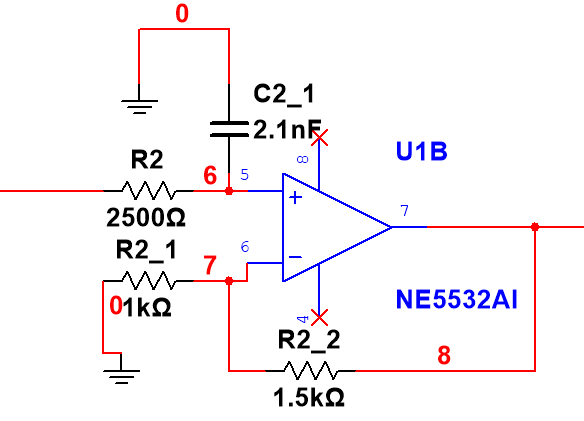
\includegraphics[width=.6\textwidth]{picture/TIM20190505131858}
  \caption{低通滤波器电路图}\label{qzzydlt11}
\end{figure}
\subsubsection{仿真情况}
借助Multisim仿真,得到线性增益情况见图\ref{qzzyfzt112}
。\par 可知其基本符合通带2.5倍增益的要求。
\begin{figure}[htbp]
  \centering
  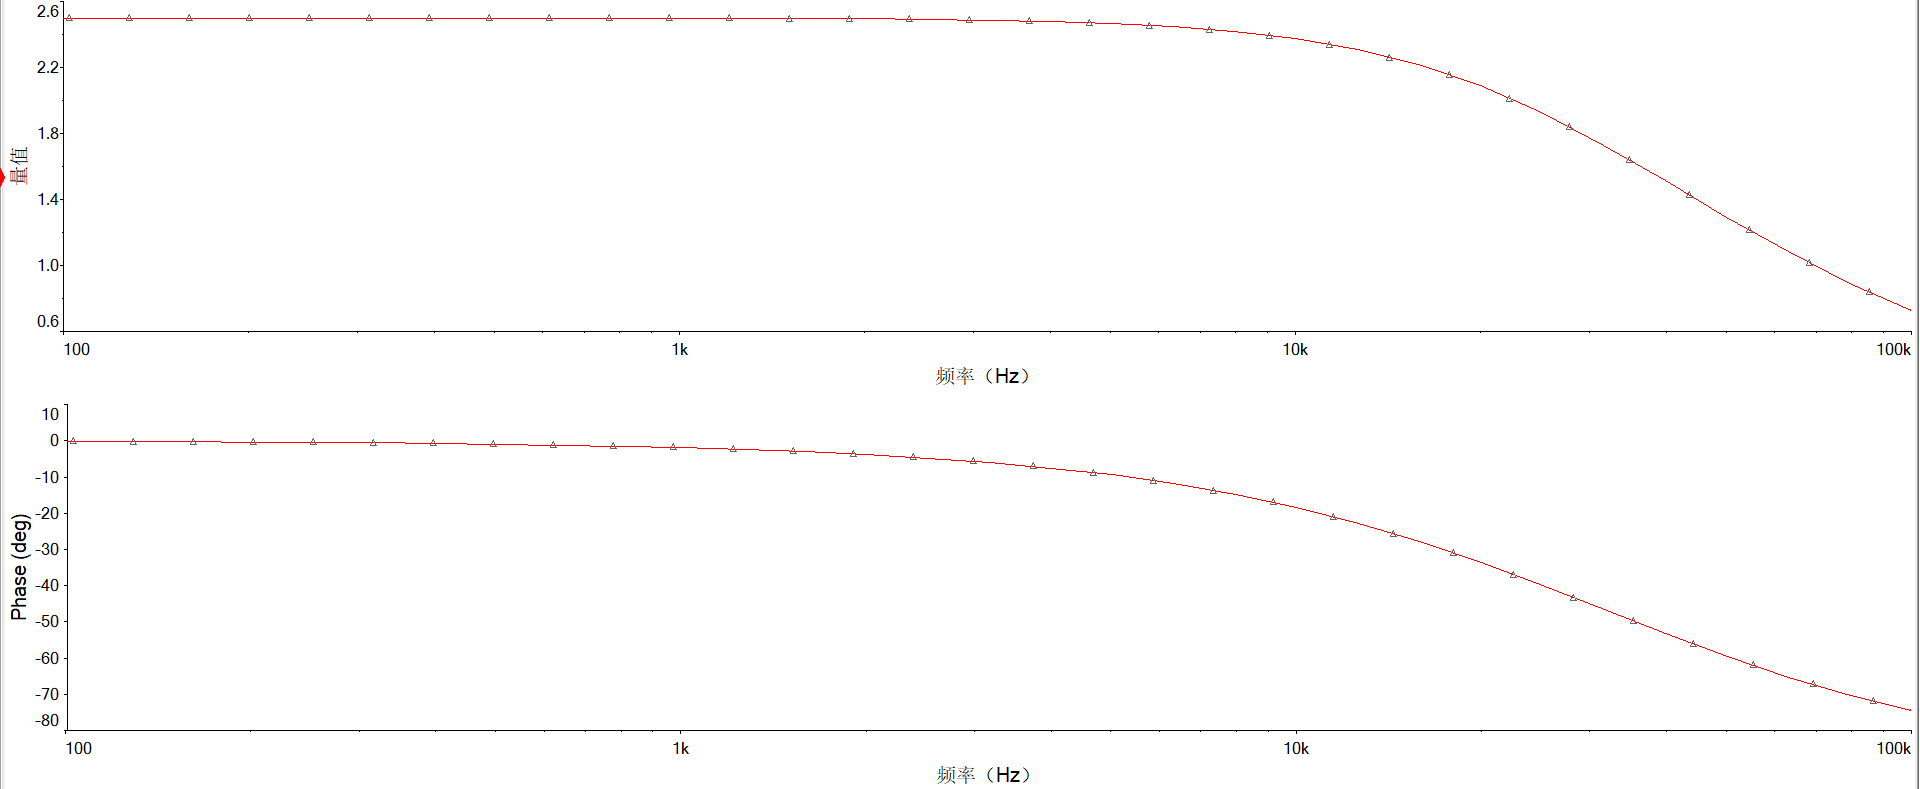
\includegraphics[width=\textwidth]{picture/TIM20190505132307}\\
  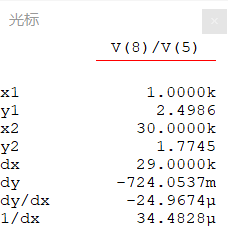
\includegraphics[width=.3\textwidth]{picture/TIM20190505132403}
  \caption{低通滤波器仿真情况(线性)}\label{qzzyfzt112}
\end{figure}\par而分贝增益情况见图\ref{qzzyfzt1121}
。\par 可知其基本符合3dB截止频率为30KHZ的要求,当$f>f_p$时,曲线以$-20dB$/十倍频下降。
\begin{figure}[htbp]
  \centering
  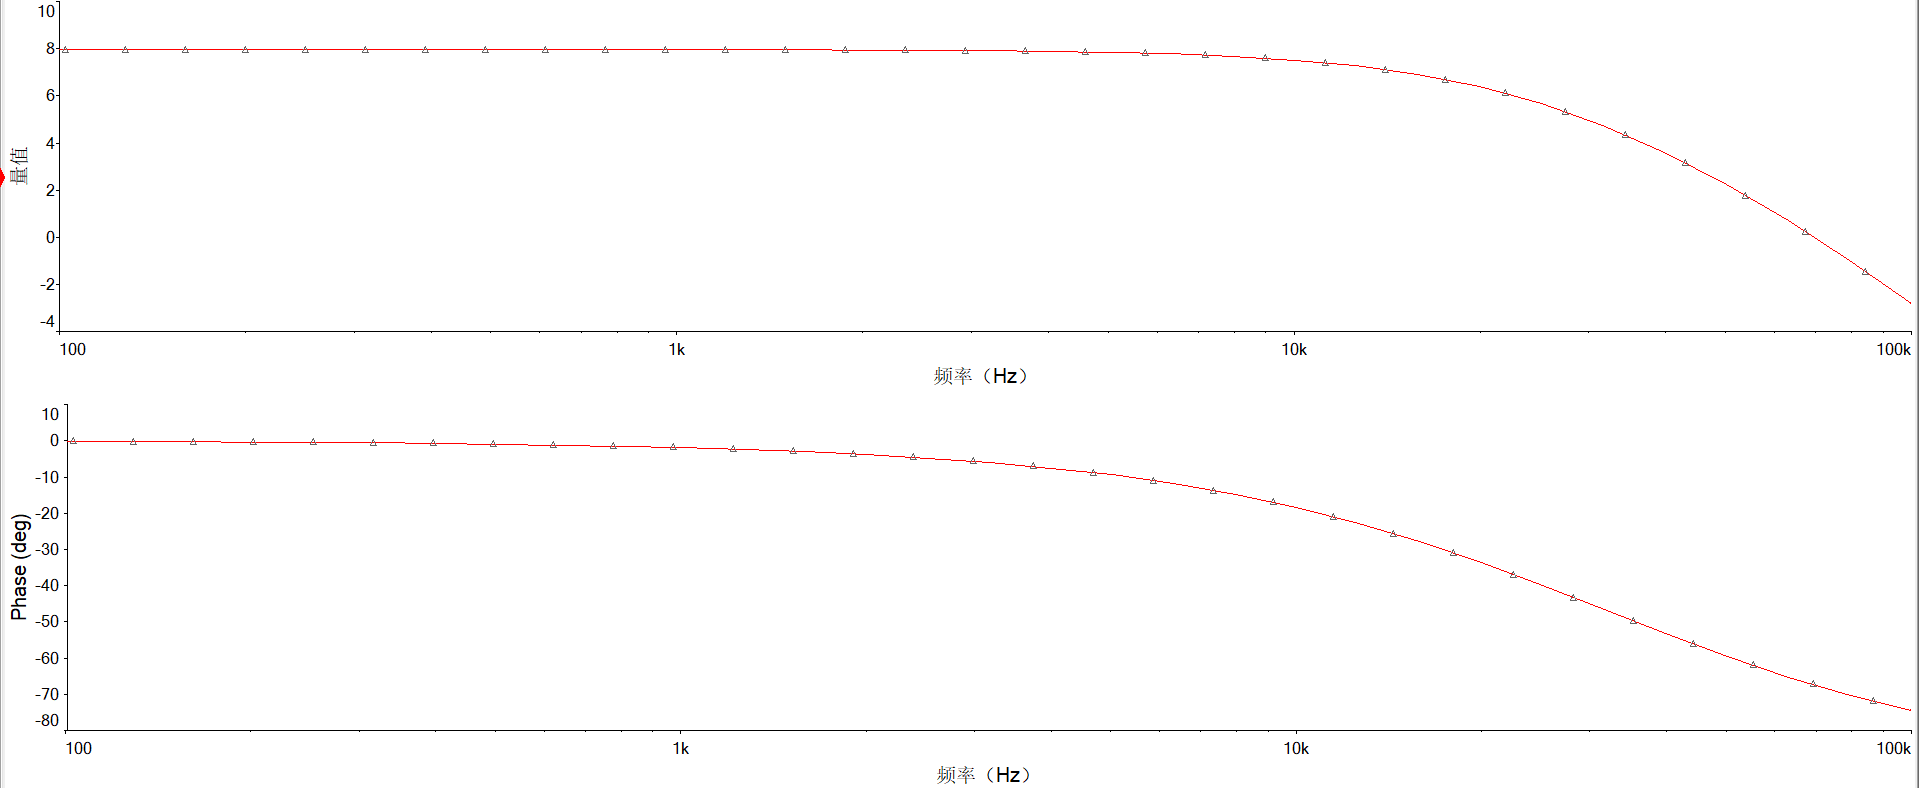
\includegraphics[width=\textwidth]{picture/TIM20190505132825}\\
  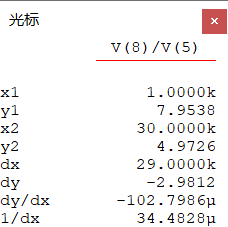
\includegraphics[width=.3\textwidth]{picture/TIM20190505132907}
  \caption{低通滤波器仿真情况(分贝)}\label{qzzyfzt1121}
\end{figure}
\subsection{压控电压源二阶高通滤波器电路}
\subsubsection{电路原理}
如图\ref{yjdtlbq11}
\begin{figure}[htbp]
  \centering
  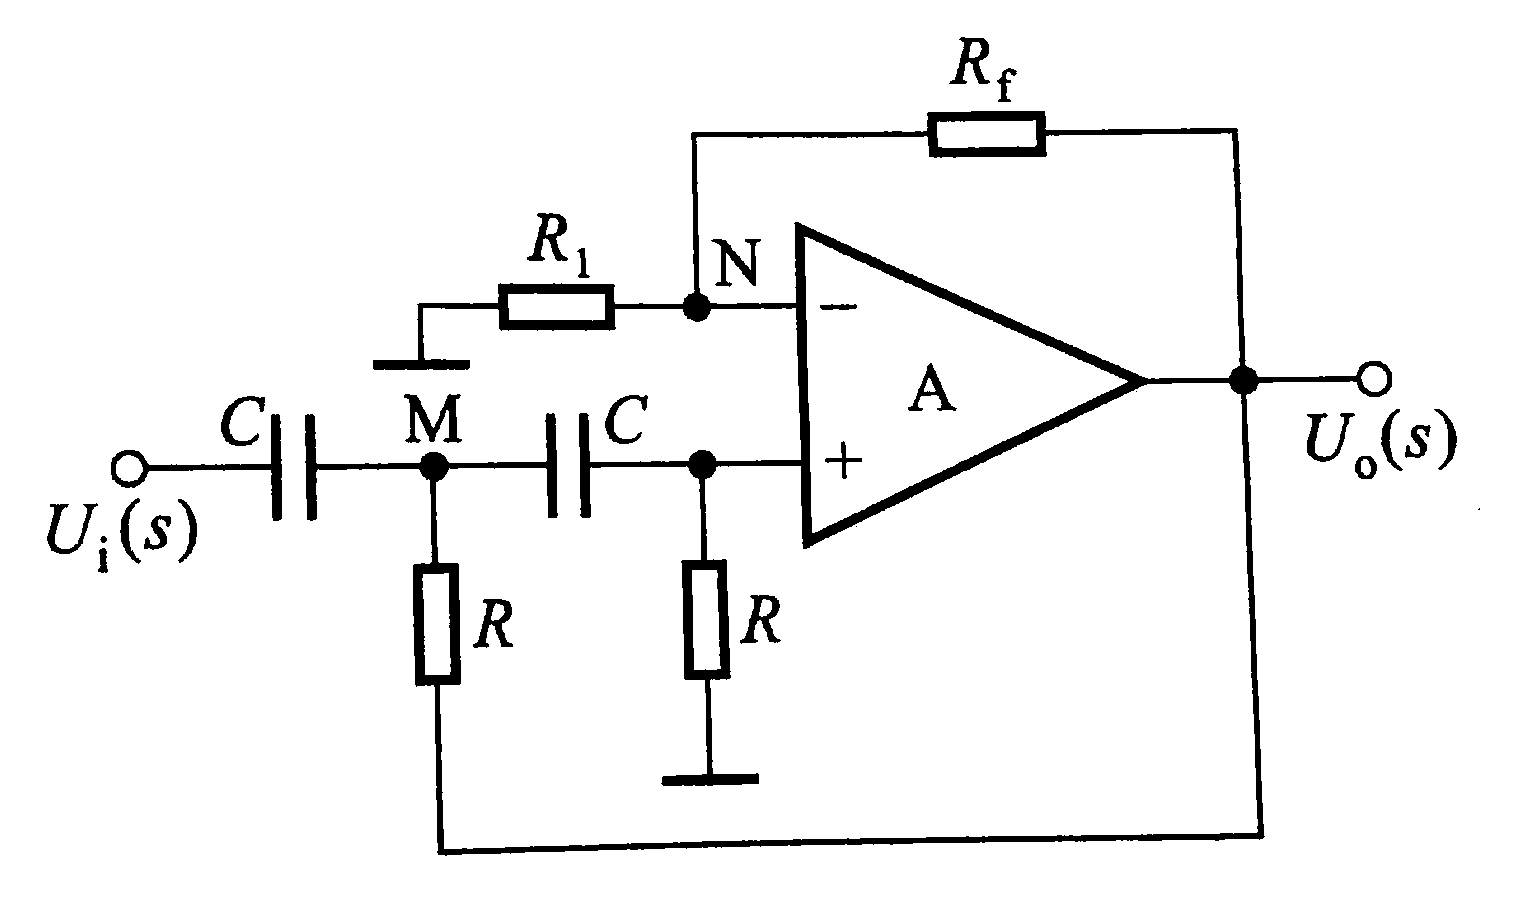
\includegraphics[width=.5\textwidth]{picture/P3}
  \caption{压控电压源二阶高通滤波器电路原理}\label{yjdtlbq11}
\end{figure}
,电路的传递函数、通带放大倍数、截止频率和品质因数分别为
\begin{gather}
		A_u(s)=A_{up}(s)\cdot\frac{sRC^2}{1+\left[3-A_{up}(s)\right]sRC+\left(sRC\right)^2}\\
		\dot{A}_{up}=1+\frac{R_f}{R_1}\\
        f_p=\frac{1}{2\pi RC}\\
        Q=\frac{1}{3-\dot{A}_{up}}
	\end{gather}\par
为实现2倍通带增益、3dB截止频率为1KHZ,取$\frac{R_f}{R_1}=1$,$f_p=1KHZ$,于是$R=120\Omega$,$C=1.2\mu F$
。\par
但仿真时,发现以上的取值并不能使3dB截止频率为1KHZ,于是最终调整后的取值中,$R=100\Omega$。
\subsubsection{Multisim电路图}
由电路原理,得到电路图如图\ref{qzzydlt1133}
。
\begin{figure}[htbp]
  \centering
  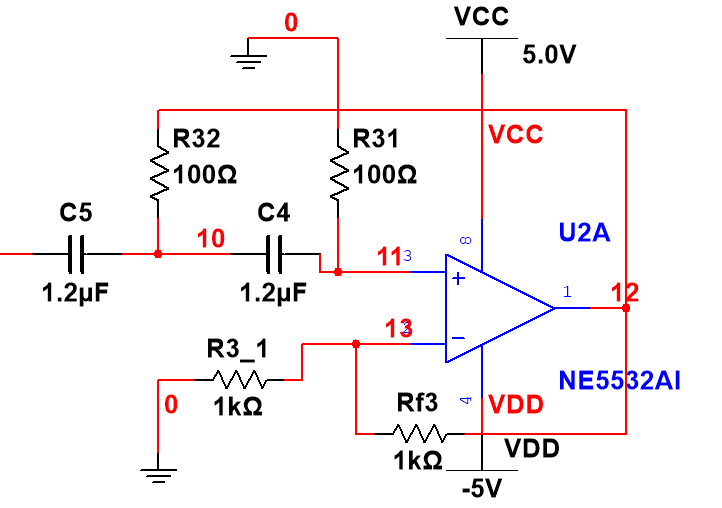
\includegraphics[width=.6\textwidth]{picture/TIM20190505134645}
  \caption{高通滤波器电路图}\label{qzzydlt1133}
\end{figure}
\subsubsection{仿真情况}
借助Multisim仿真,得到线性增益情况见图\ref{qzzyfzt11233}
。\par 可知其基本符合通带2倍增益的要求。
\begin{figure}[htbp]
  \centering
  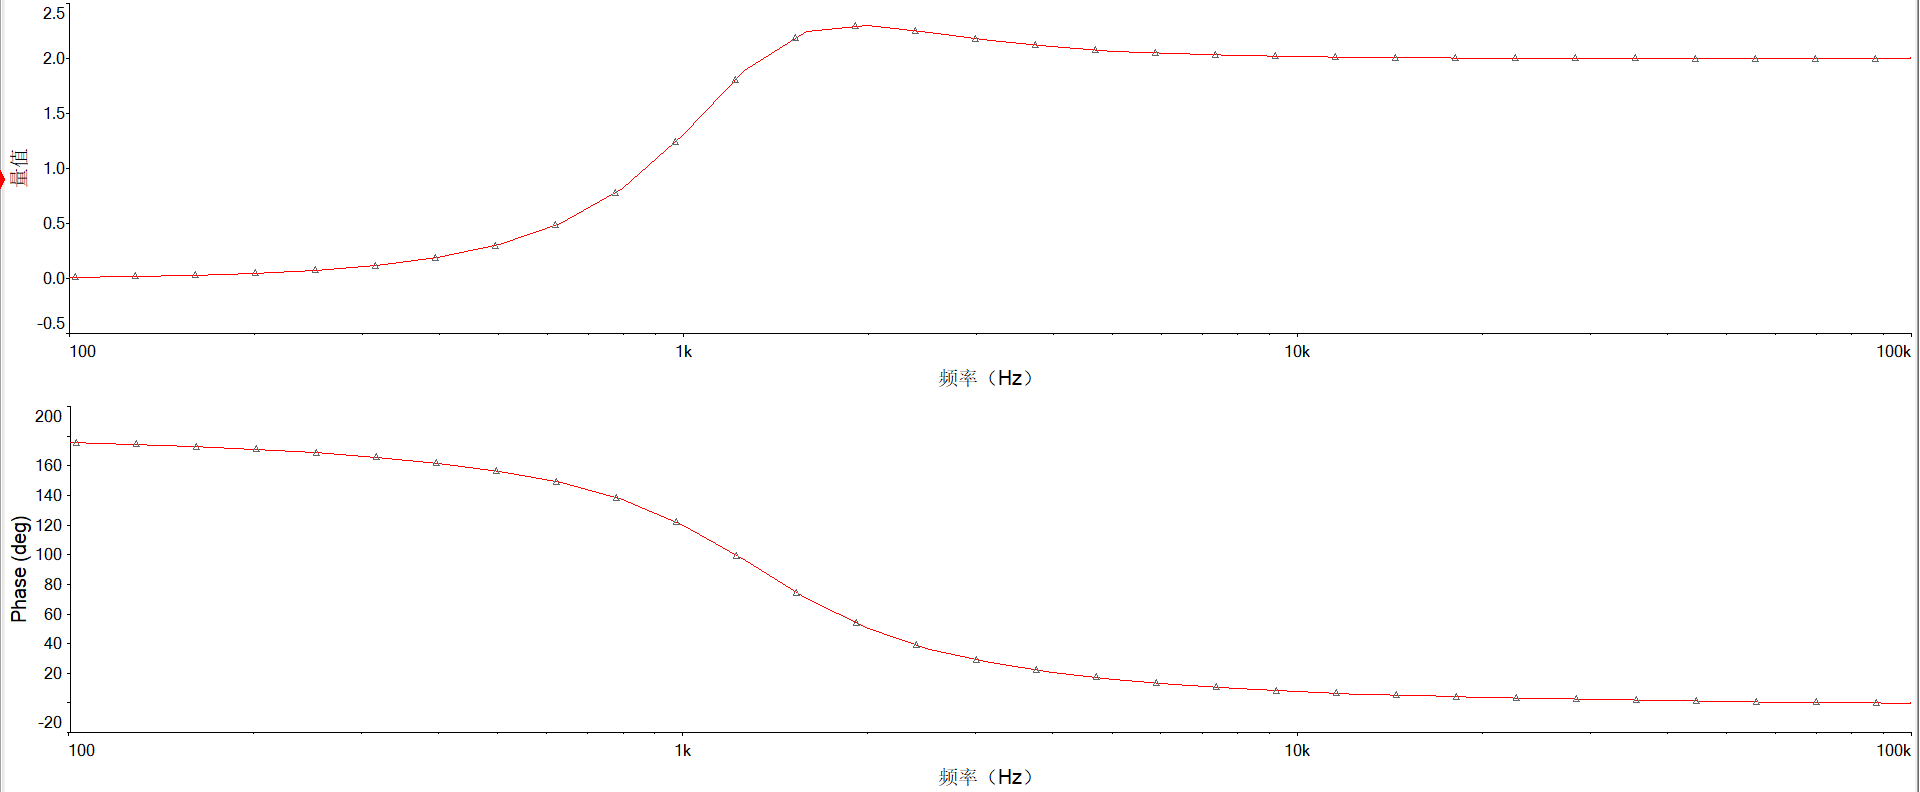
\includegraphics[width=\textwidth]{picture/TIM20190505134845}\\
  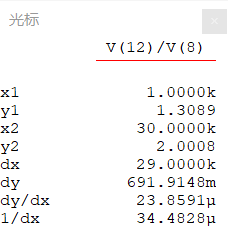
\includegraphics[width=.3\textwidth]{picture/TIM20190505134934}
  \caption{高通滤波器仿真情况(线性)}\label{qzzyfzt11233}
\end{figure}\par而分贝增益情况见图\ref{qzzyfzt112133}
。\par 可知其基本符合3dB截止频率为1KHZ的要求。
\begin{figure}[htbp]
  \centering
  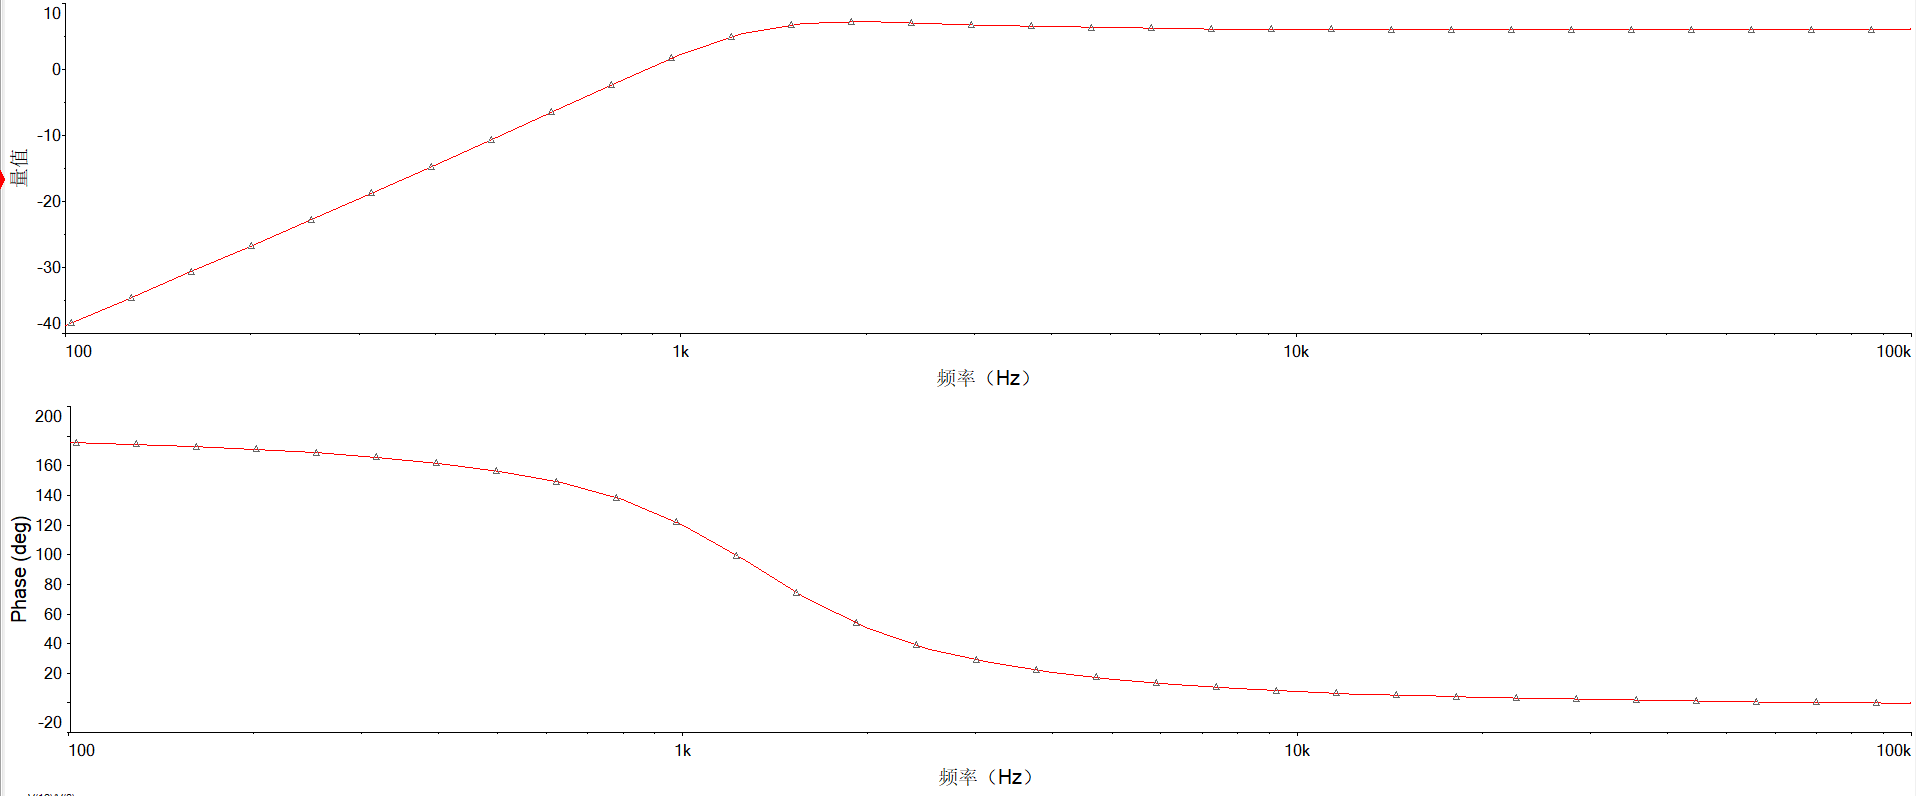
\includegraphics[width=\textwidth]{picture/TIM20190505135202}\\
  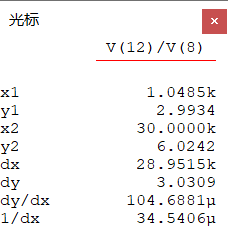
\includegraphics[width=.3\textwidth]{picture/TIM20190505135251}
  \caption{高通滤波器仿真情况(分贝)}\label{qzzyfzt112133}
\end{figure}
\section{电路总系统}
\setcounter{equation}{0}
\setcounter{table}{0}
\setcounter{figure}{0}
\subsection{电路总图}
将以上子电路级联,得到总电路图如图\ref{all}
。
\begin{figure}[htbp]
  \centering
  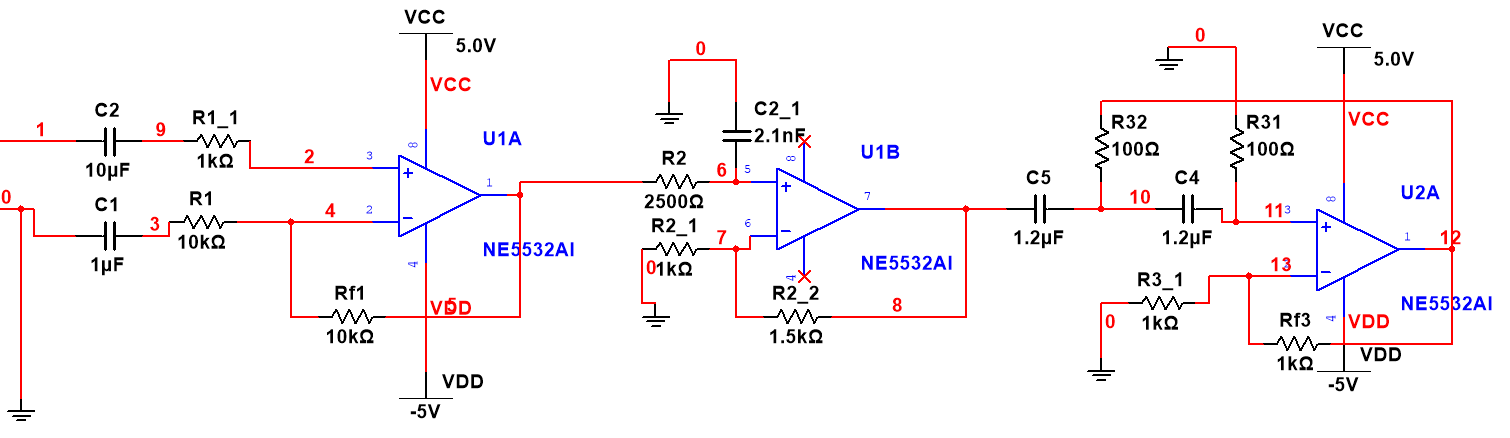
\includegraphics[width=\textwidth]{picture/TIM20190505135556}
  \caption{总电路图}\label{all}
\end{figure}
\subsection{Multisim仿真}
借助Multisim仿真,得到增益情况见图\ref{allfz}
。\par
可知其基本符合要求,增益为20dB,3dB上限截止频率为1KHZ,3dB下限截止频率为30KHZ。
\begin{figure}[htbp]
  \centering
  \begin{tabular}{cc}
    \multicolumn{2}{c}{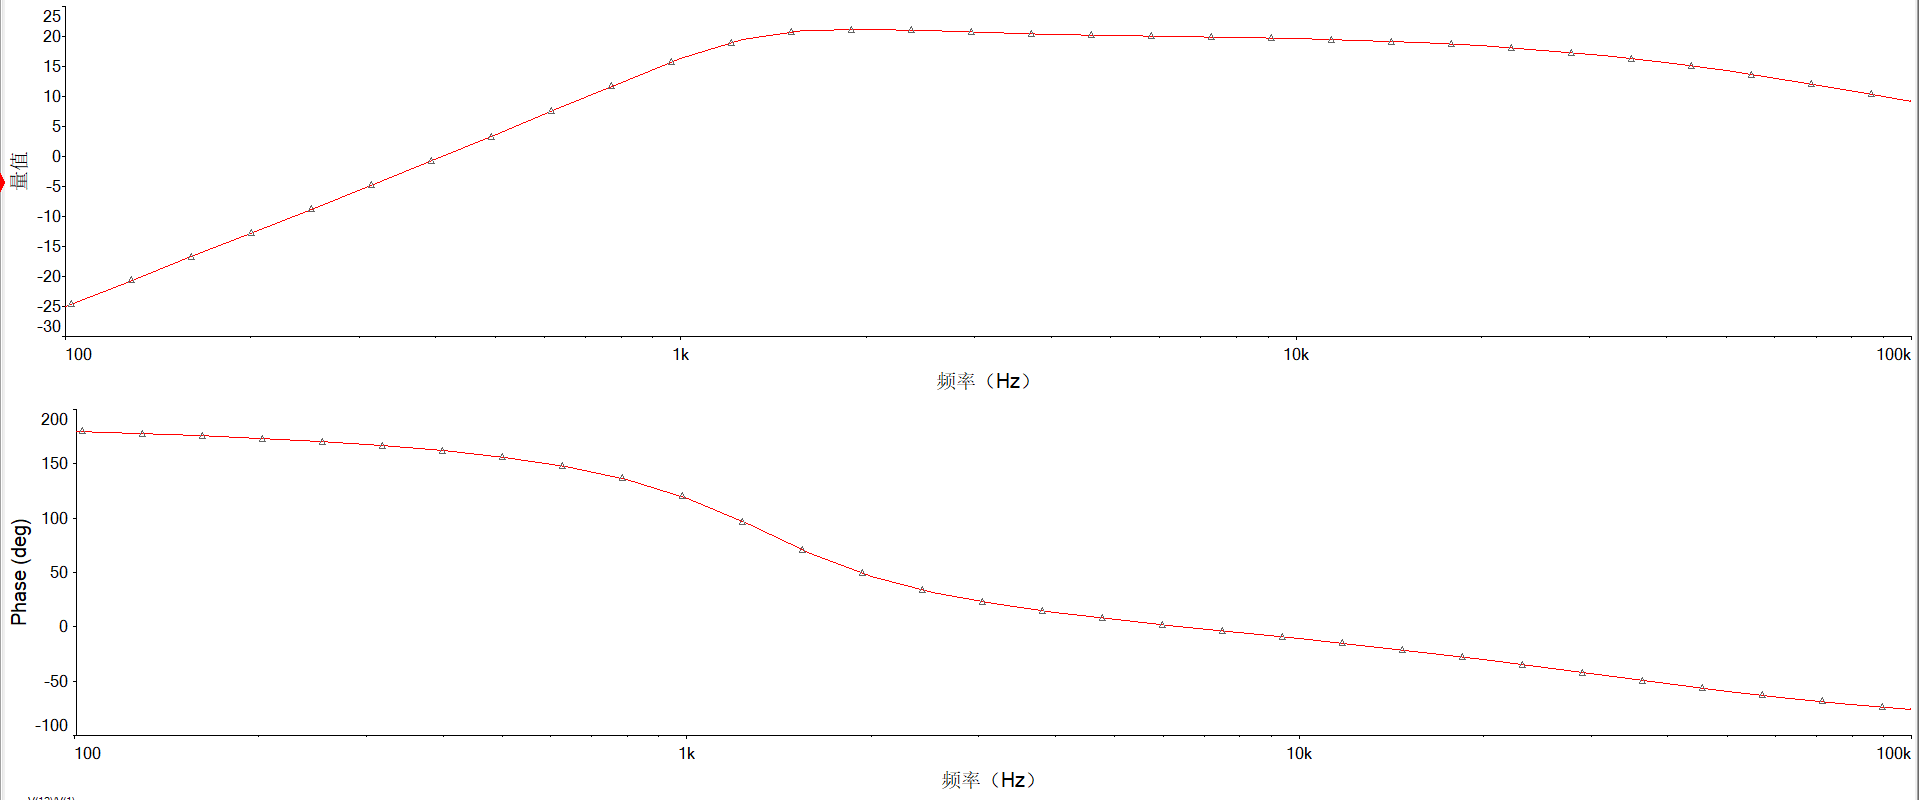
\includegraphics[width=\textwidth]{picture/TIM20190505140154}} \\
    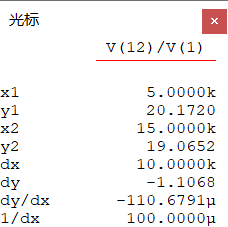
\includegraphics[width=0.3\textwidth]{picture/TIM20190505140252} & 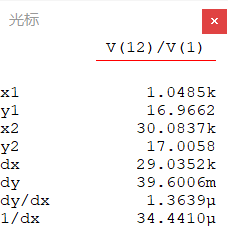
\includegraphics[width=0.3\textwidth]{picture/TIM20190505140428} \\
  \end{tabular}
  \caption{总仿真情况}\label{allfz}
\end{figure}
\end{document}
